%
% tikztemplate.tex -- Template für standalone TIKZ Bilder
%
% (c) 2019 Prof Dr Andreas Müller, Hochschule Rapperswil
%
\documentclass[tikz,12pt]{standalone}
\usepackage{amsmath}
\usepackage{times}
\usepackage{txfonts}
\usepackage{pgfplots}
\usepackage{csvsimple}
\usetikzlibrary{arrows,intersections,math}
\begin{document}
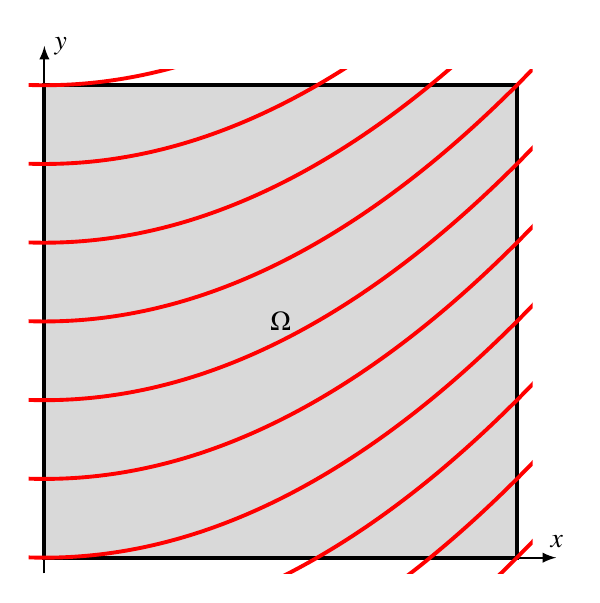
\begin{tikzpicture}[>=latex]

\fill[color=gray!30] (0,0)--(6,0)--(6,6)--(0,6)--cycle;

\draw[->,line width=0.7pt] (-0.2,0)--(6.5,0) coordinate[label=$x$];
\draw[->,line width=0.7pt] (0,-0.2)--(0,6.5) coordinate[label={right:$y$}];

\draw[line width=1.4pt] (0,0)--(6,0)--(6,6)--(0,6)--cycle;

\begin{scope}
\clip (-0.2,-0.2) rectangle (6.2,6.2);
\foreach \a in {-3,...,6}{
	\draw[color=red,line width=1.4pt] plot[domain=-0.3:6.3,samples=100]
		({\x},{(6/2)*(\x/6)*(\x/6)+\a});
}
\end{scope}

\node at (3,3) {$\Omega$};

\end{tikzpicture}
\end{document}

